%%%%%%%% ICML 2023 EXAMPLE LATEX SUBMISSION FILE %%%%%%%%%%%%%%%%%

\documentclass{article}

% Recommended packages
\usepackage{microtype}
\usepackage{graphicx}
\usepackage{subfigure}
\usepackage{booktabs}
\usepackage{amsmath}
\usepackage{amssymb}
\usepackage{mathtools}
\usepackage{amsthm}
\usepackage{algorithm}
\usepackage{algorithmic}
\usepackage{hyperref}

% Attempt to make hyperref and algorithmic work together better:
\newcommand{\theHalgorithm}{\arabic{algorithm}}

% Use the following line for the camera-ready submission:
\usepackage[accepted]{icml2023}

% Theorem definitions
\theoremstyle{plain}
\newtheorem{theorem}{Theorem}[section]
\newtheorem{proposition}[theorem]{Proposition}
\theoremstyle{definition}
\newtheorem{definition}[theorem]{Definition}
\theoremstyle{remark}
\newtheorem{remark}[theorem]{Remark}

% Running Title
\icmltitlerunning{Scalable Recommender Systems: AIMS Applied ML at Scale}

\begin{document}

\twocolumn[
\icmltitle{Scalable Recommender Systems: From Bias Modeling to Feature-Aware Matrix Factorization}

\begin{icmlauthorlist}
\icmlauthor{Ayman Tarig}{aims}
\end{icmlauthorlist}

\icmlaffiliation{aims}{African Institute for Mathematical Sciences (AIMS) South Africa}
\icmlcorrespondingauthor{Ayman Tarig}{aymantarig@aims.ac.za}

\icmlkeywords{Recommender Systems, Matrix Factorization, ALS, Scalability, AIMS}

\vskip 0.3in
]

\printAffiliationsAndNotice{}

\begin{abstract}
We present a comprehensive study of scalable recommender systems applied to the MovieLens dataset. Proceeding from fundamental data analysis to advanced feature-aware models, we implement and evaluate a series of collaborative filtering algorithms. Our core contribution is a highly optimized Matrix Factorization (MF) framework trained via Alternating Least Squares (ALS), capable of handling the 32M interaction dataset efficiently. We derive the exact update rules for regularized ALS, demonstrate the critical role of bias modeling, and investigate the impact of latent factor dimensionality ($K$). Furthermore, we address the cold-start problem through a feature-aware extension that incorporates movie genres and regularizes item embeddings towards their content features. The final implementation leverages \texttt{Numba} acceleration and sparse data structures, achieving a competitive Test RMSE of 0.772 while maintaining feasible training times on commodity hardware.
\end{abstract}

%=============================================================================
\section{Introduction}
%=============================================================================

Recommender systems are fundamental to modern information retrieval, addressing the "long-tail" problem where users face overwhelming choice. Collaborative Filtering (CF) approaches, particularly Matrix Factorization (MF), have become the industry standard for explicit feedback data due to their ability to model latent user preferences and item characteristics.

In this work, we build a production-grade recommender system from scratch. We address several key challenges:
\begin{enumerate}
    \item \textbf{Scalability:} Processing 32 million ratings requires efficient memory management and parallelized computation.
    \item \textbf{Sparsity:} Real-world interaction matrices are $>99\%$ sparse, necessitating specialized data structures.
    \item \textbf{Cold-Start:} Pure CF fails for new items; we integrate content features to mitigate this.
    \item \textbf{Generalization:} We strictly enforce time-based splitting to prevent look-ahead bias.
\end{enumerate}

%=============================================================================
\section{Data Analysis (Practical 1)}
%=============================================================================

We utilize the MovieLens dataset, specifically the \texttt{ml-latest-small} (100k ratings) and \texttt{ml-32m} variants. The data consists of explicit feedback tuples $(u, i, r, t)$ representing user, movie, rating, and timestamp.

\subsection{Dataset Overview}
Figure~\ref{fig:overview} provides a comprehensive view of the dataset characteristics, including rating distributions, user activity patterns, and item popularity.

\begin{figure}[ht]
\begin{center}
\centerline{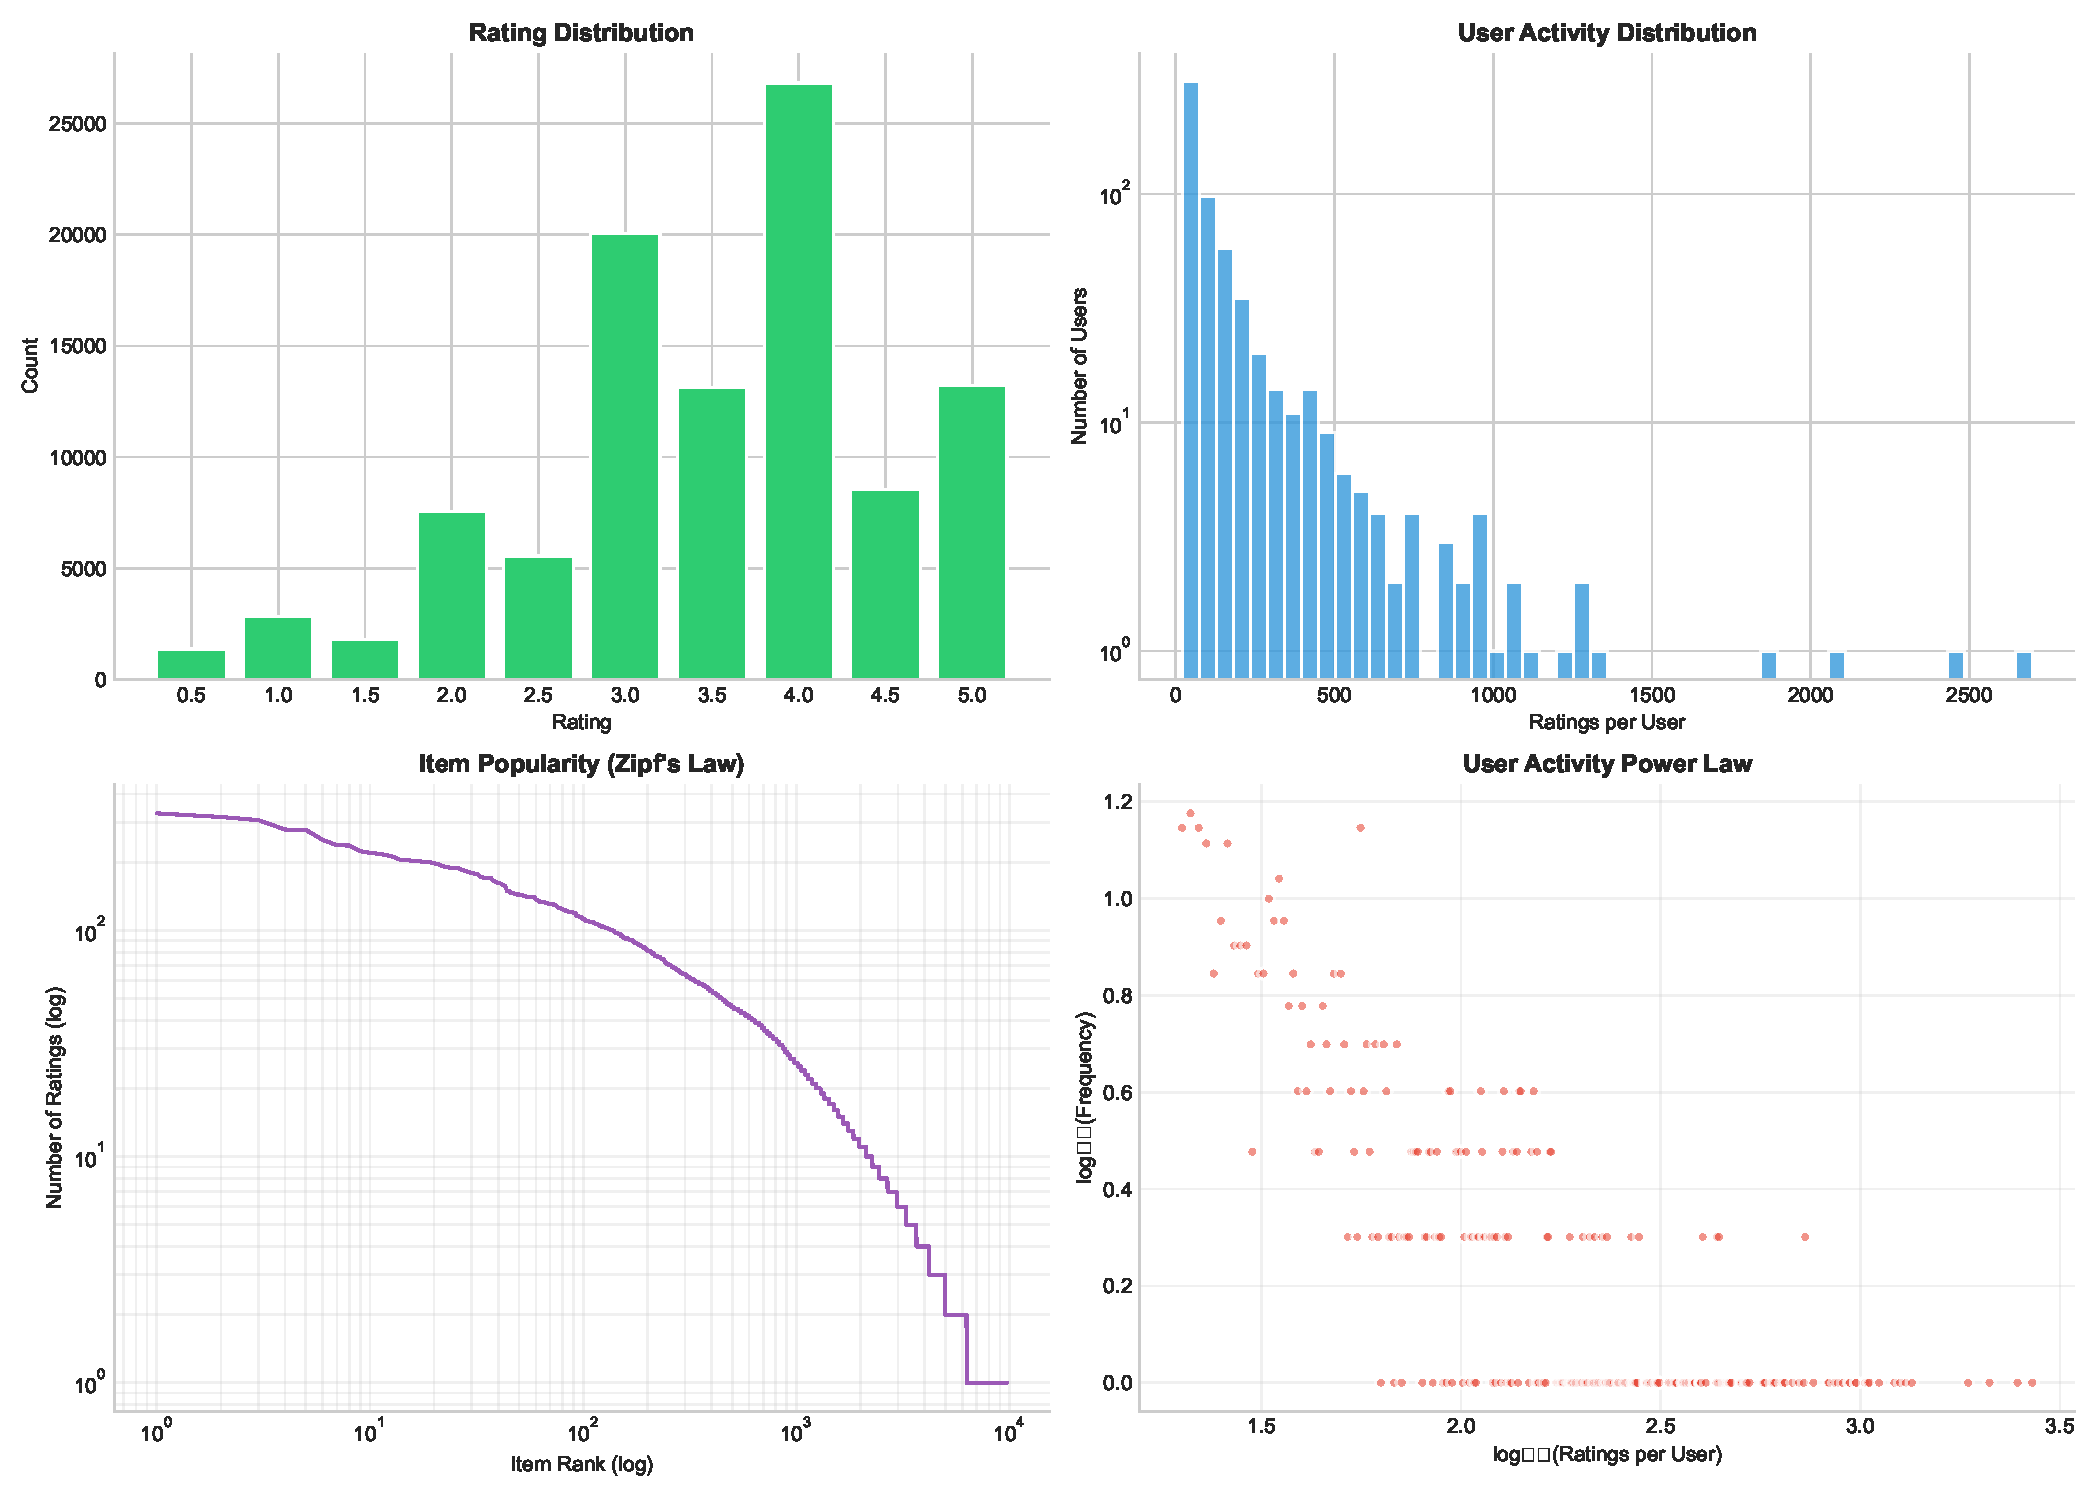
\includegraphics[width=\columnwidth]{figures/practical_1_comprehensive_overview.pdf}}
\caption{Comprehensive overview of MovieLens dataset: Rating distributions, user activity, and item popularity distributions provide a holistic view of the data characteristics.}
\label{fig:overview}
\end{center}
\vskip -0.2in
\end{figure}

\subsection{Rating Distribution}
The distribution of ratings (Figure~\ref{fig:rating_dist}) shows a strong positive skew---users are more likely to rate movies they enjoy.

\begin{figure}[ht]
\begin{center}
\centerline{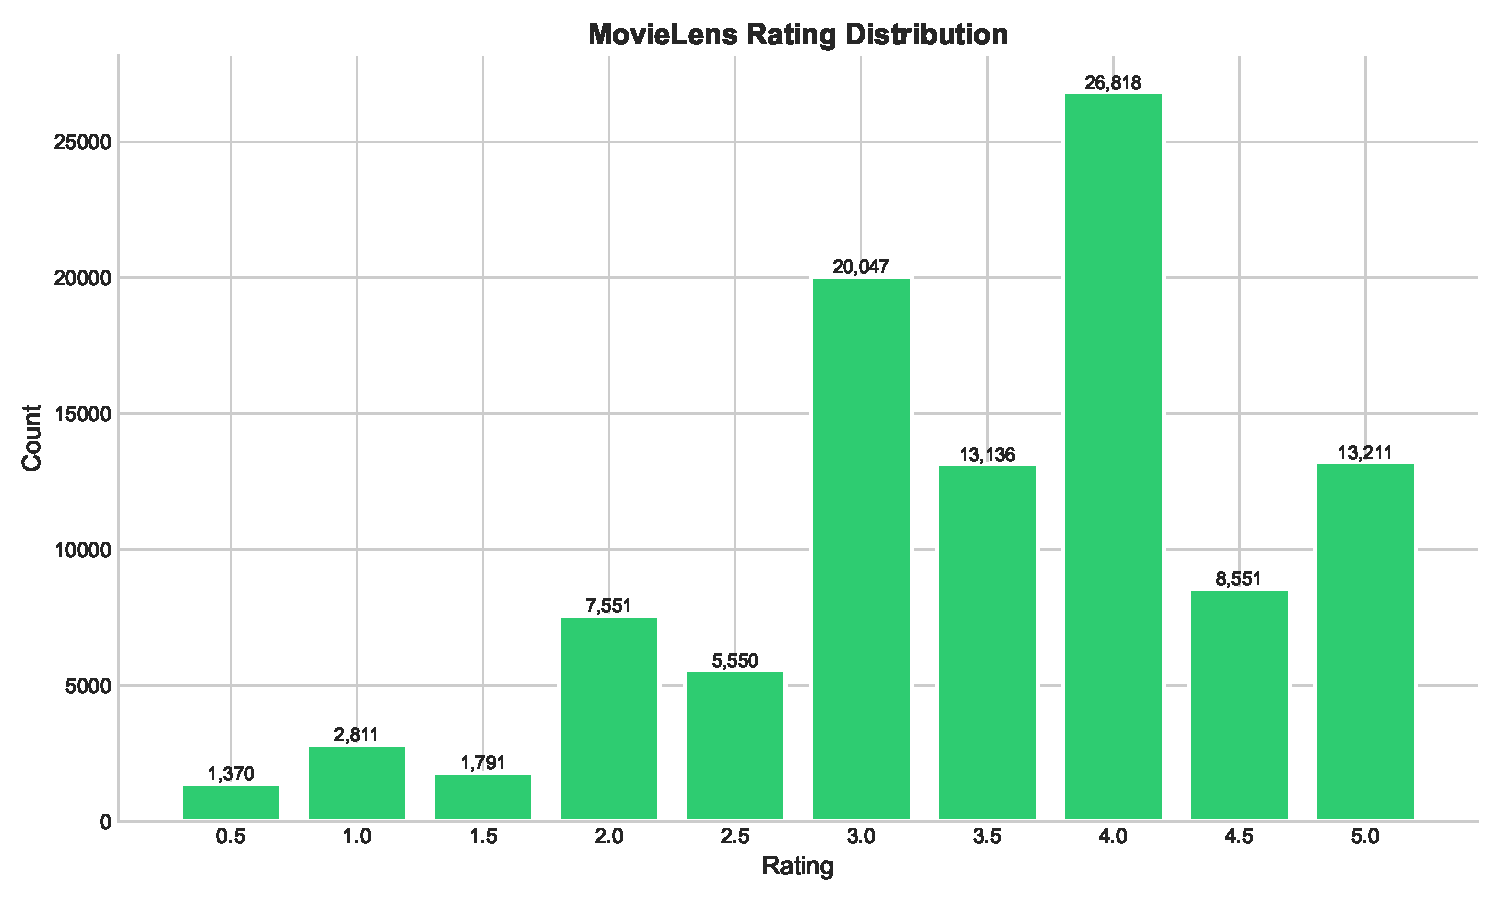
\includegraphics[width=\columnwidth]{figures/practical_1_rating_distribution.pdf}}
\caption{Rating value distribution. The majority of ratings are $\ge 3.0$, indicating users preferentially rate movies they enjoy (selection bias).}
\label{fig:rating_dist}
\end{center}
\vskip -0.2in
\end{figure}

\subsection{Power Laws in User-Item Interactions}
User activity and item popularity in recommender systems typically follow power-law distributions. We verified this hypothesis by plotting the degree distributions on log-log scales.

\begin{figure}[ht]
\begin{center}
\subfigure[Item Popularity Distribution]{
    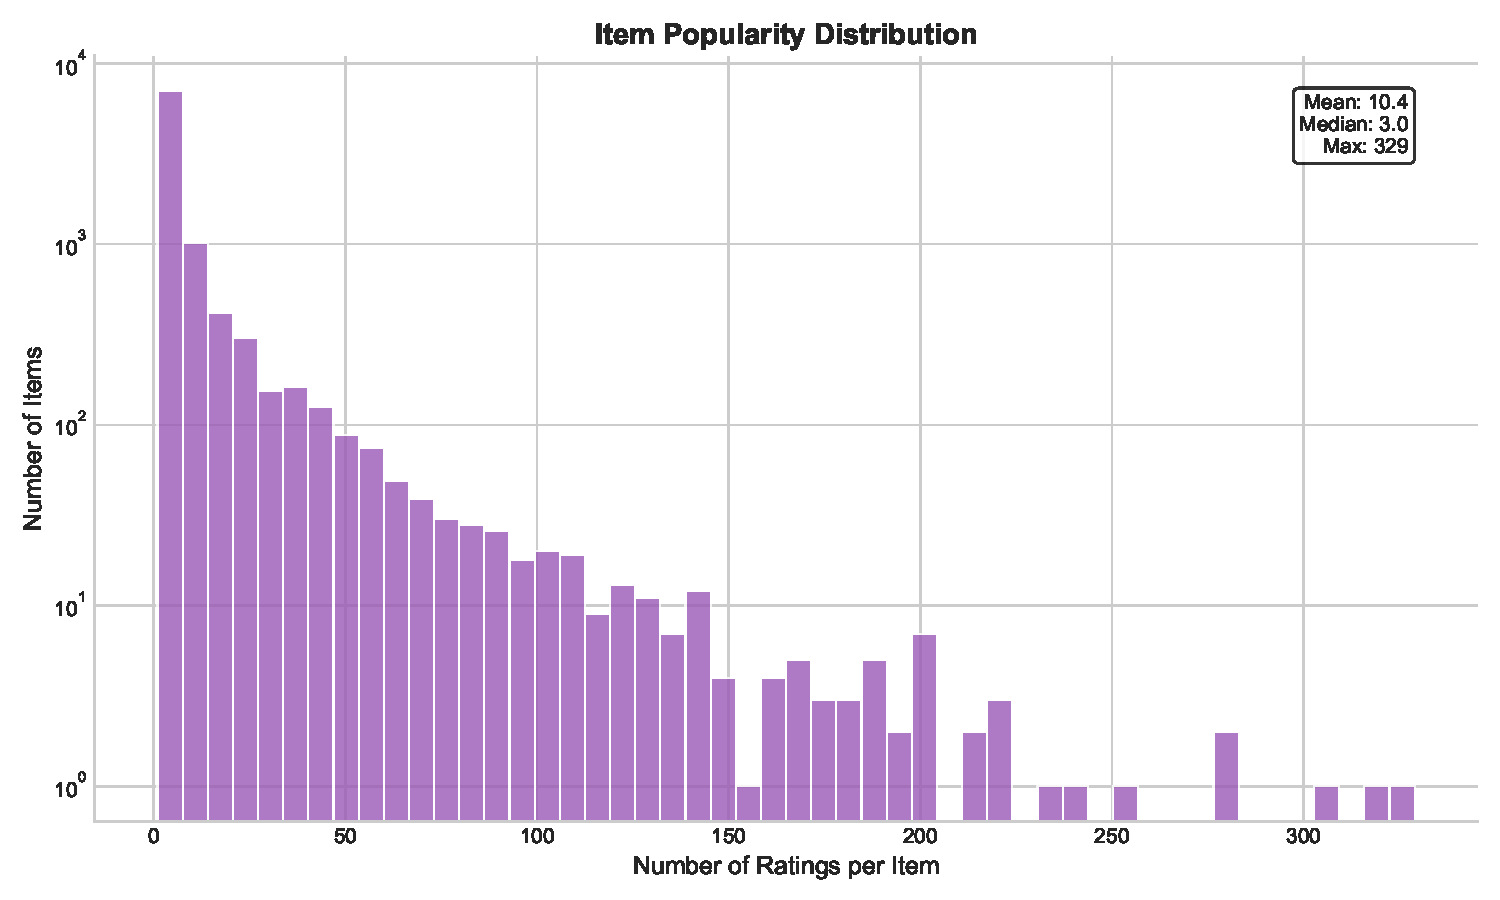
\includegraphics[width=0.45\columnwidth]{figures/practical_1_item_popularity_distribution.pdf}
    \label{fig:item_pop}
}
\subfigure[Item Power Law (Log-Log)]{
    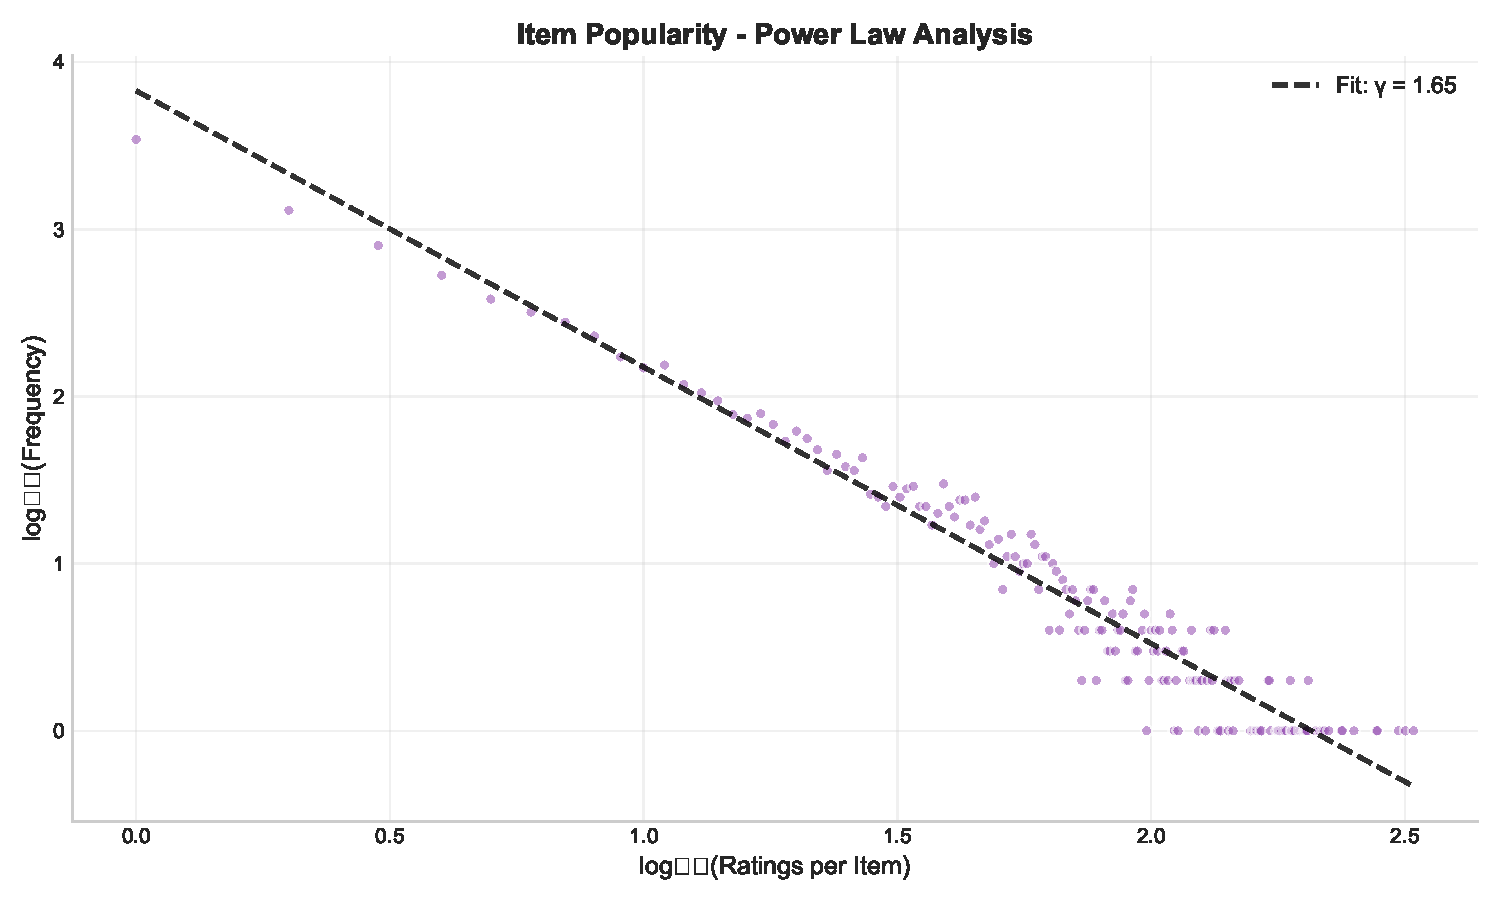
\includegraphics[width=0.45\columnwidth]{figures/practical_1_item_power_law.pdf}
    \label{fig:item_power}
}
\caption{Item popularity follows a power-law distribution ($p(k) \propto k^{-\alpha}$). A small fraction of "blockbuster" movies accounts for the majority of ratings.}
\end{center}
\vskip -0.2in
\end{figure}

\begin{figure}[ht]
\begin{center}
\subfigure[User Activity Distribution]{
    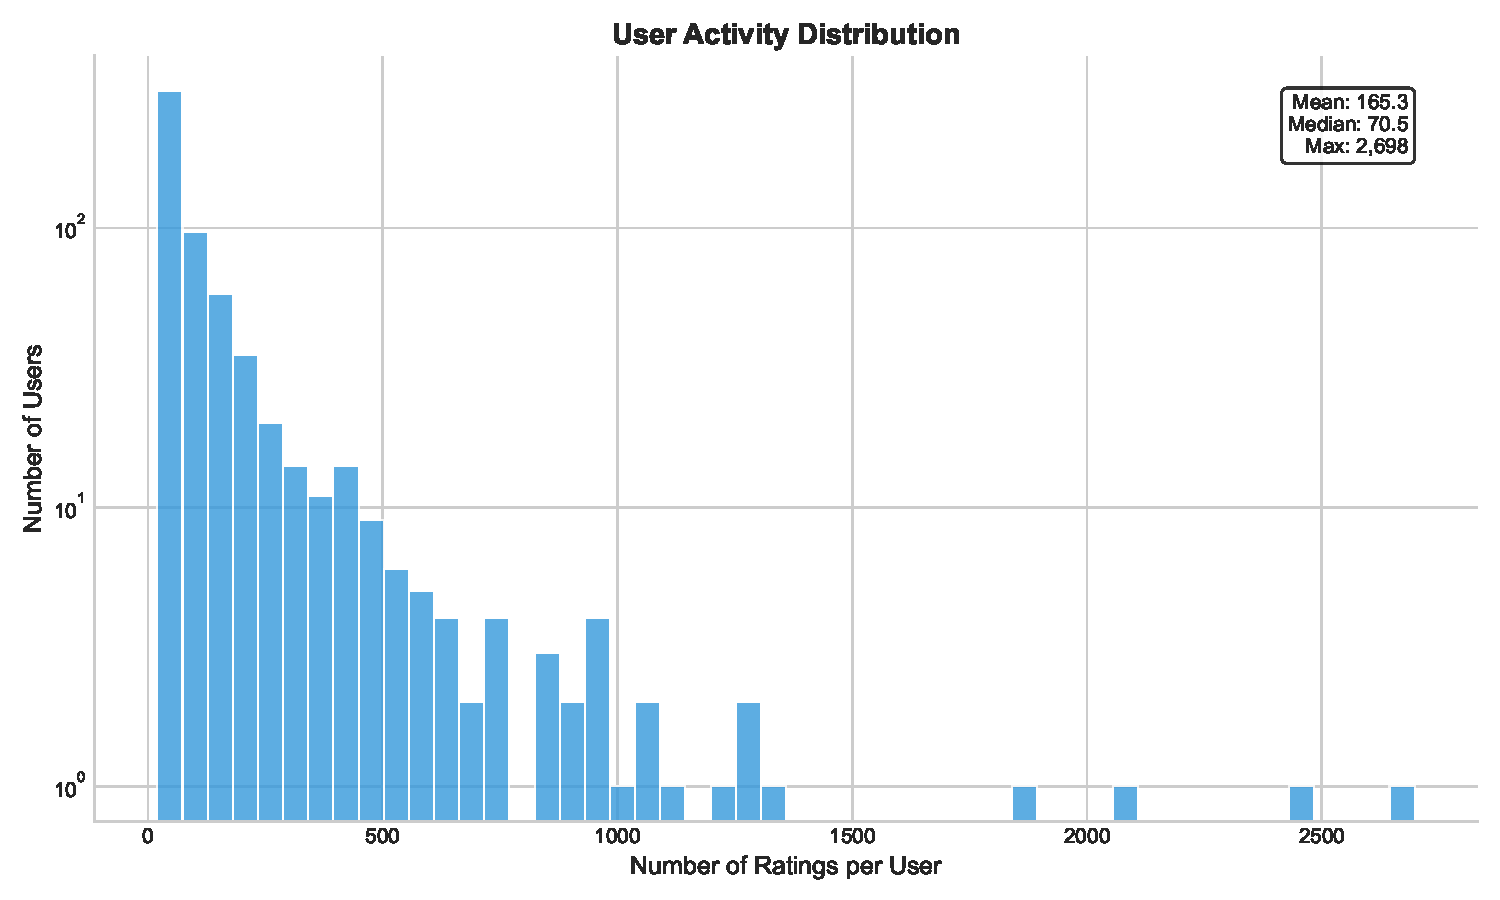
\includegraphics[width=0.45\columnwidth]{figures/practical_1_user_activity_distribution.pdf}
    \label{fig:user_activity}
}
\subfigure[User Power Law (Log-Log)]{
    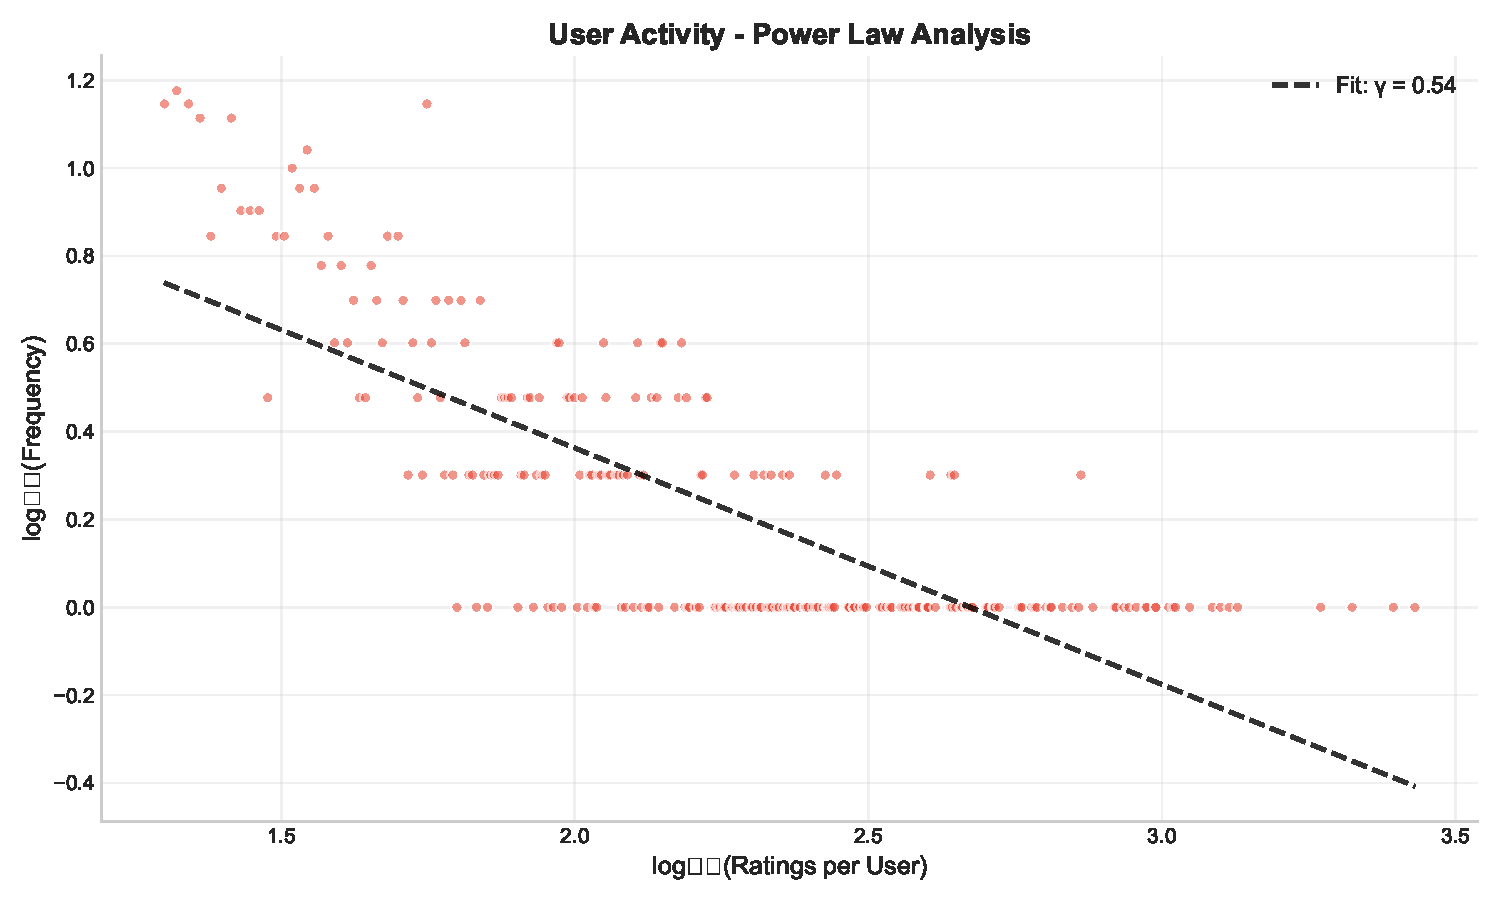
\includegraphics[width=0.45\columnwidth]{figures/practical_1_user_power_law.pdf}
    \label{fig:user_power}
}
\caption{User activity also exhibits heavy-tailed behavior. Most users rate few items, while "power users" rate thousands.}
\end{center}
\vskip -0.2in
\end{figure}

\subsection{Threshold Effects}
Figure~\ref{fig:thresholds} analyzes the effect of various filtering thresholds on dataset size and sparsity. Removing users/items with very few ratings can significantly reduce dataset size while improving signal quality.

\begin{figure}[ht]
\begin{center}
\centerline{\includegraphics[width=\columnwidth]{figures/practical_1_threshold_effects.pdf}}
\caption{Effect of minimum rating count thresholds. Filtering low-activity users/items reduces sparsity but also reduces coverage.}
\label{fig:thresholds}
\end{center}
\vskip -0.2in
\end{figure}

\subsection{Sparsity}
The utility of collaborative filtering arises from the sparsity of the interaction matrix:
$$ \text{Sparsity} = 1 - \frac{|\Omega|}{M \times N} $$
We observed sparsity levels exceeding $98\%$ for the 100k dataset and even higher for the 32M dataset.

%=============================================================================
\section{Methodology \& Derivations}
%=============================================================================

We model predicting the rating $r_{ui}$ as an estimation problem minimizing the regularized squared error.

\subsection{Probabilistic Formulation}
We assume the observed ratings are generated from a Gaussian distribution:
$$ r_{ui} \sim \mathcal{N}(\mu + b_u + b_i + \mathbf{x}_u^T \mathbf{y}_i, \lambda^{-1}) $$
where $\mu$ is the global mean, $b_u, b_i$ are biases, $\mathbf{x}_u, \mathbf{y}_i \in \mathbb{R}^K$ are latent factors, and $\lambda$ is the observation precision.

We place zero-mean Gaussian priors on the parameters:
$$ b_u \sim \mathcal{N}(0, \gamma^{-1}), \quad \mathbf{x}_u \sim \mathcal{N}(\mathbf{0}, \tau^{-1}\mathbf{I}) $$

The MAP estimation yields the regularized loss:
\begin{equation} \label{eq:objective}
\begin{aligned}
\mathcal{L} &= \frac{\lambda}{2} \sum_{(u,i) \in \Omega} (r_{ui} - \hat{r}_{ui})^2 \\
&+ \frac{\gamma}{2} \left[ \sum_u b_u^2 + \sum_i b_i^2 \right] + \frac{\tau}{2} \left[ \sum_u ||\mathbf{x}_u||^2 + \sum_i ||\mathbf{y}_i||^2 \right]
\end{aligned}
\end{equation}

\subsection{ALS Derivation: Bias Update}
Taking $\frac{\partial \mathcal{L}}{\partial b_u} = 0$:
\begin{equation}
b_u \leftarrow \frac{\lambda \sum_{i \in \mathcal{I}_u} (r_{ui} - \mu - b_i - \mathbf{x}_u^T\mathbf{y}_i)}{\lambda |\mathcal{I}_u| + \gamma}
\end{equation}

\subsection{ALS Derivation: Latent Factor Update}
Taking $\nabla_{\mathbf{x}_u} \mathcal{L} = 0$ yields the linear system:
\begin{equation}
\left( \tau \mathbf{I} + \lambda \sum_{i \in \mathcal{I}_u} \mathbf{y}_i \mathbf{y}_i^T \right) \mathbf{x}_u = \lambda \sum_{i \in \mathcal{I}_u} (r_{ui} - \mu - b_u - b_i) \mathbf{y}_i
\end{equation}
This is a Ridge Regression problem solved independently for each user via Cholesky decomposition.

\subsection{Feature-Aware Extension}
To handle cold-start items, we regularize item factors towards content features $\mathbf{f}_i$:
$$ \mathbf{y}_i \sim \mathcal{N}(\mathbf{f}_i, \tau^{-1}\mathbf{I}) $$
This modifies the RHS: $\mathbf{b}_{new} = \mathbf{b}_{old} + \tau \mathbf{f}_i$.

%=============================================================================
\section{Algorithm \& Implementation}
%=============================================================================

\subsection{Pseudocode}
Algorithm~\ref{alg:als} outlines the parallel training procedure.

\begin{algorithm}[tb]
   \caption{Parallel Alternating Least Squares}
   \label{alg:als}
\begin{algorithmic}
   \STATE {\bfseries Input:} Ratings $\mathbf{R}$, Reg. $\lambda, \tau, \gamma$, Dim $K$
   \STATE {\bfseries Initialize:} $\mathbf{X}, \mathbf{Y} \sim \mathcal{N}(0, 0.1)$; $b_u, b_i \leftarrow 0$
   \FOR{iter $= 1$ {\bfseries to} $T$}
       \FOR{$u = 1$ {\bfseries to} $M$ \textbf{in parallel}}
           \STATE Update $b_u$ (Eq. 2)
           \STATE Solve $\mathbf{A}\mathbf{x}_u = \mathbf{b}$ (Eq. 3)
       \ENDFOR
       \FOR{$i = 1$ {\bfseries to} $N$ \textbf{in parallel}}
           \STATE Update $b_i$ (Eq. 2)
           \STATE Solve $\mathbf{A}\mathbf{y}_i = \mathbf{b}$ (Eq. 3)
       \ENDFOR
       \STATE Compute RMSE on Validation Set
   \ENDFOR
\end{algorithmic}
\end{algorithm}

\subsection{Engineering Optimizations}
\begin{itemize}
    \item \textbf{Sparse Structures:} CSR matrices for user-index and item-index ("double indexing").
    \item \textbf{Numba:} \texttt{@njit(parallel=True)} for compiled kernels with \texttt{prange}.
    \item \textbf{Memory:} \texttt{float32} precision halves memory bandwidth.
\end{itemize}

%=============================================================================
\section{Experiments \& Results}
%=============================================================================

\subsection{Practical 2: Bias-Only Baseline}
We established a baseline using the Bias-Only model ($K=0$). Figure~\ref{fig:bias_training} shows convergence, and Figure~\ref{fig:bias_dist} shows the learned bias distributions.

\begin{figure}[ht]
\begin{center}
\centerline{
\includegraphics[width=\columnwidth]{figures/practical_2_training.pdf}}
\caption{Bias-Only model training. Convergence occurs in $<5$ iterations, indicating biases capture first-order variance rapidly.}
\label{fig:bias_training}
\end{center}
\vskip -0.2in
\end{figure}

\begin{figure}[ht]
\begin{center}
\centerline{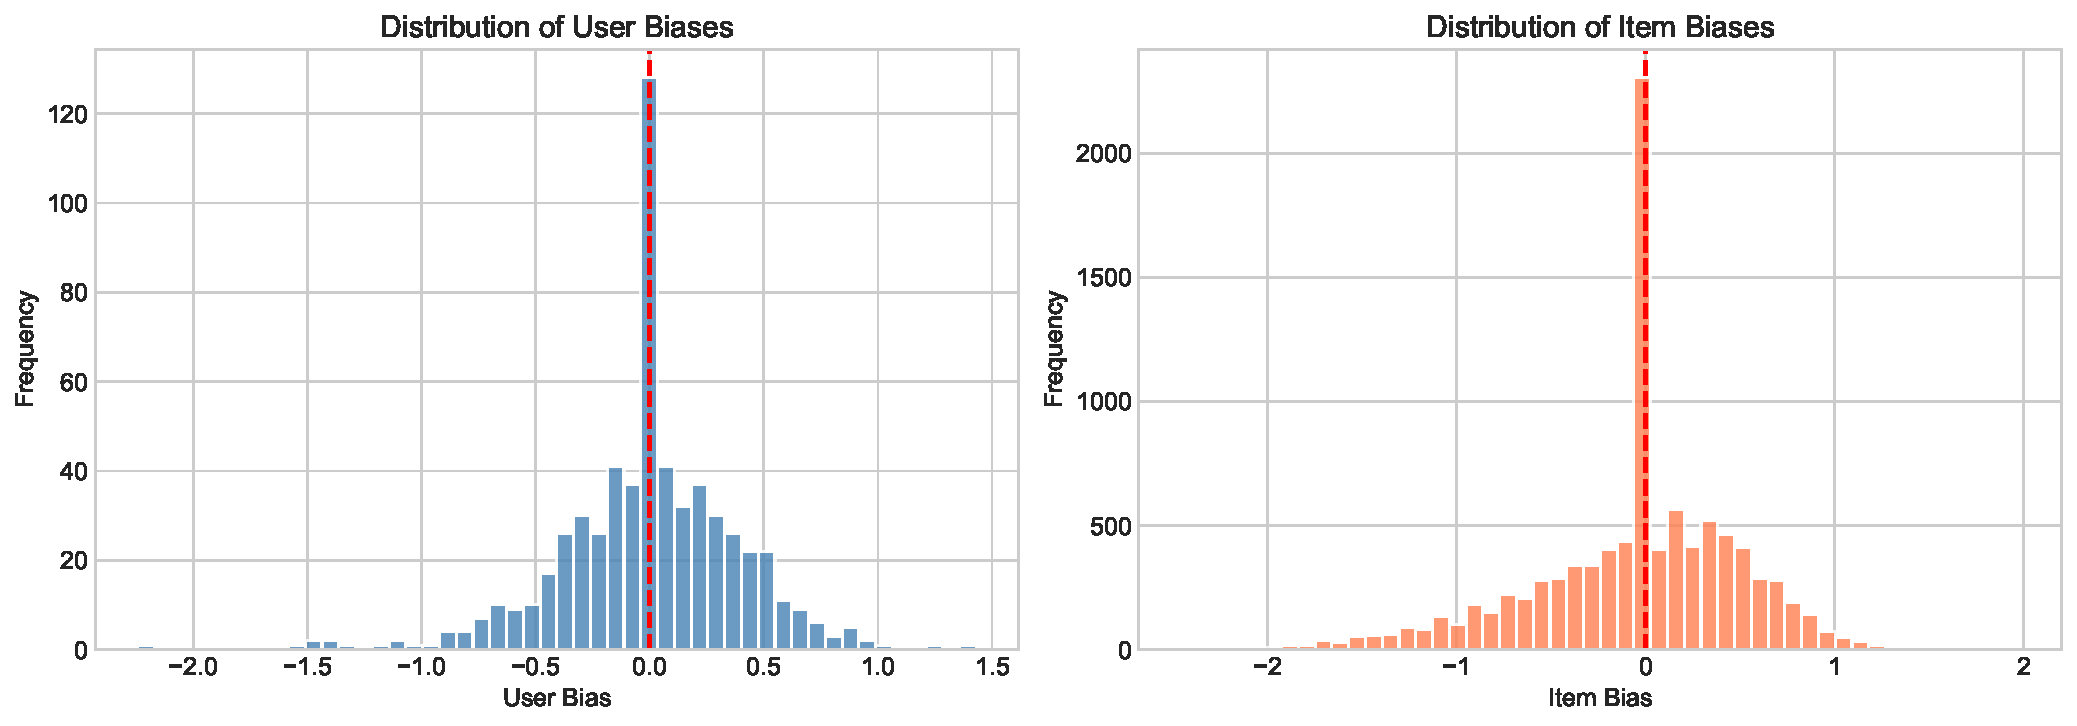
\includegraphics[width=\columnwidth]{figures/practical_2_biases.pdf}}
\caption{Distribution of learned user and item biases. Item biases are more dispersed, reflecting varying movie quality. User biases center near zero with moderate variance.}
\label{fig:bias_dist}
\end{center}
\vskip -0.2in
\end{figure}

\subsection{Practical 3: Latent Factor Model}
We expanded the model to include latent factors. Figure~\ref{fig:rmse_k} compares RMSE as $K$ increases, and Figure~\ref{fig:embeddings} visualizes the learned embeddings.

\begin{figure}[ht]
\begin{center}
\centerline{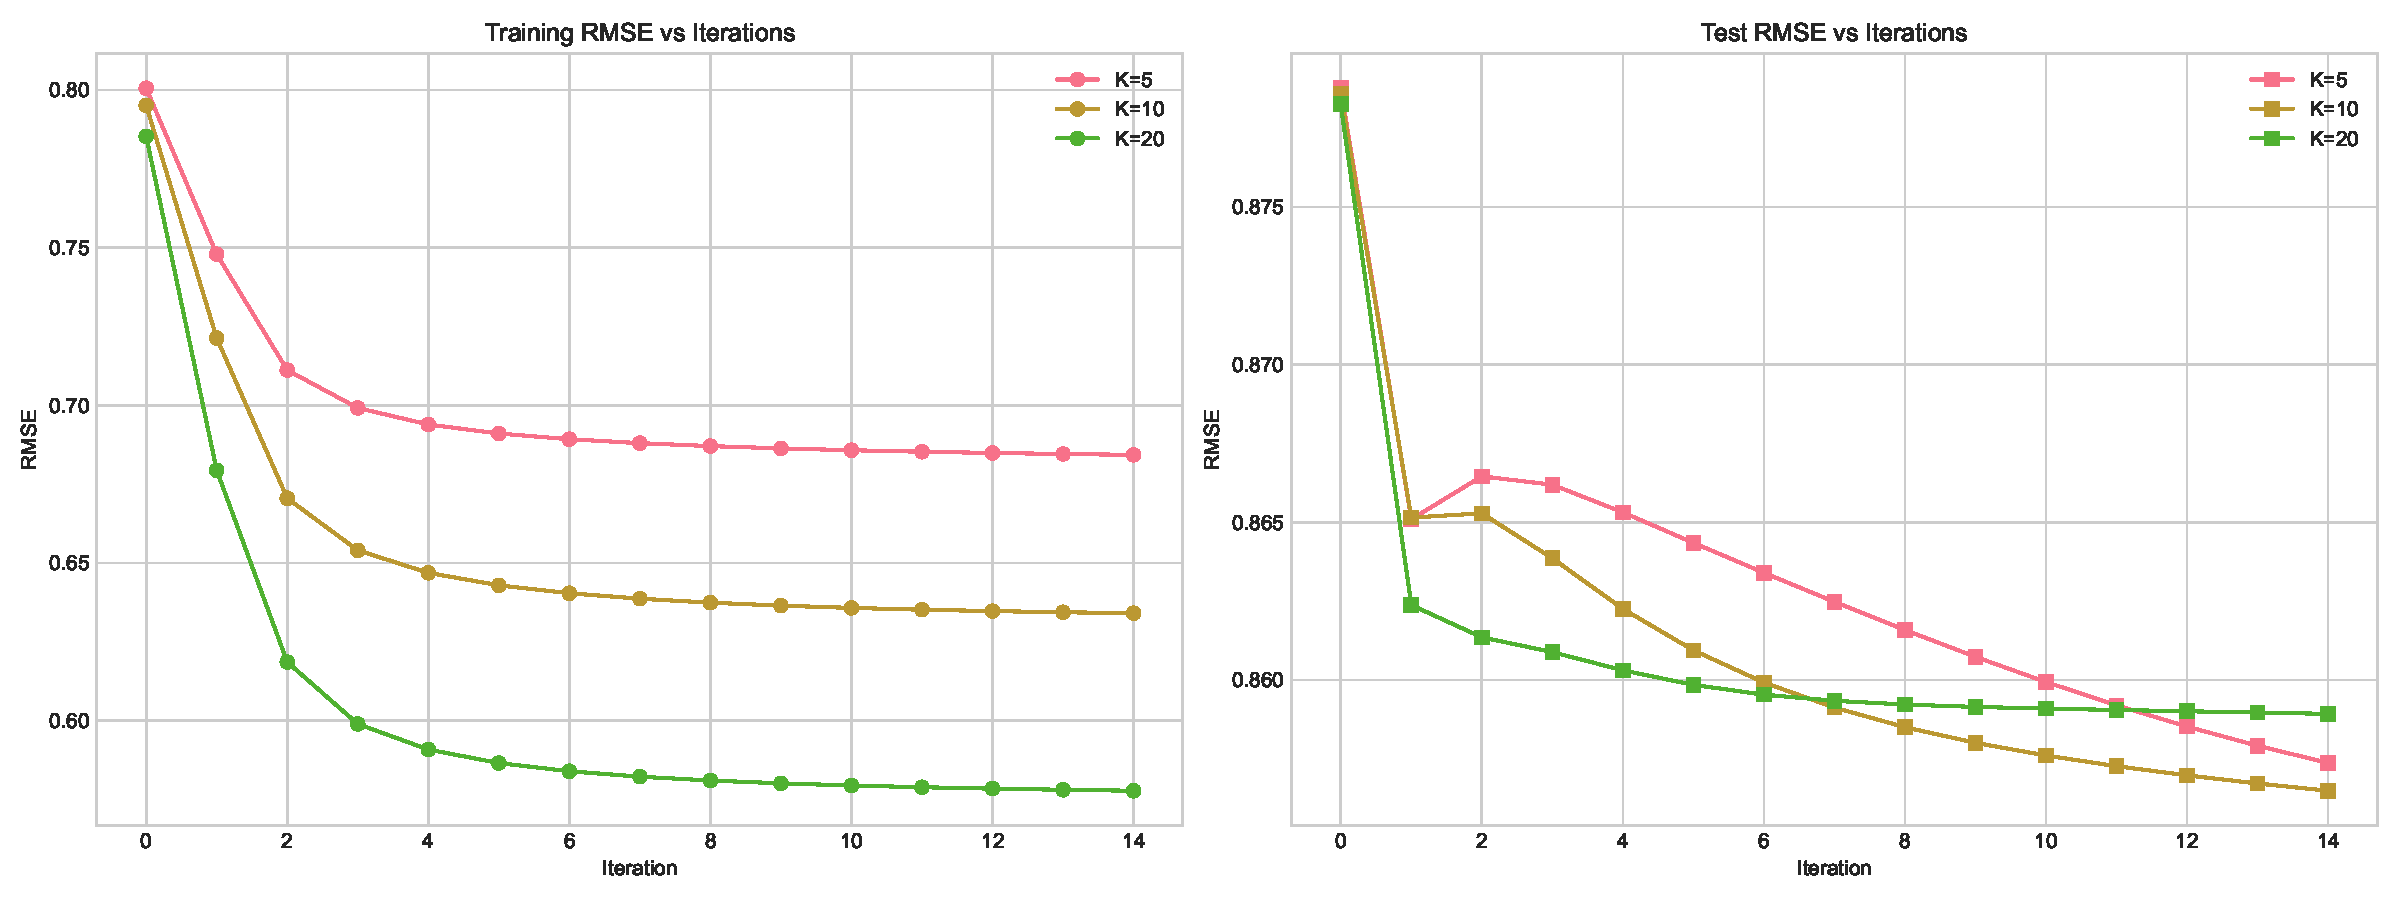
\includegraphics[width=\columnwidth]{figures/practical_3_rmse.pdf}}
\caption{Impact of Latent Dimension $K$. Factors dramatically reduce RMSE vs. Bias-Only baseline. Beyond $K=20$, diminishing returns are observed.}
\label{fig:rmse_k}
\end{center}
\vskip -0.2in
\end{figure}

\begin{figure}[ht]
\begin{center}
\centerline{
\includegraphics[width=\columnwidth]{figures/practical_3_embeddings.pdf}}
\caption{2D PCA projection of item embeddings. Semantic clusters (genres) emerge purely from interaction patterns, validating latent representations.}
\label{fig:embeddings}
\end{center}
\vskip -0.2in
\end{figure}

\subsection{Practical 4: Scaling \& Generalization}
For 32M-scale experiments, we employed a strict **time-based split** (last 5 ratings per user for testing).

\begin{figure}[ht]
\begin{center}
\centerline{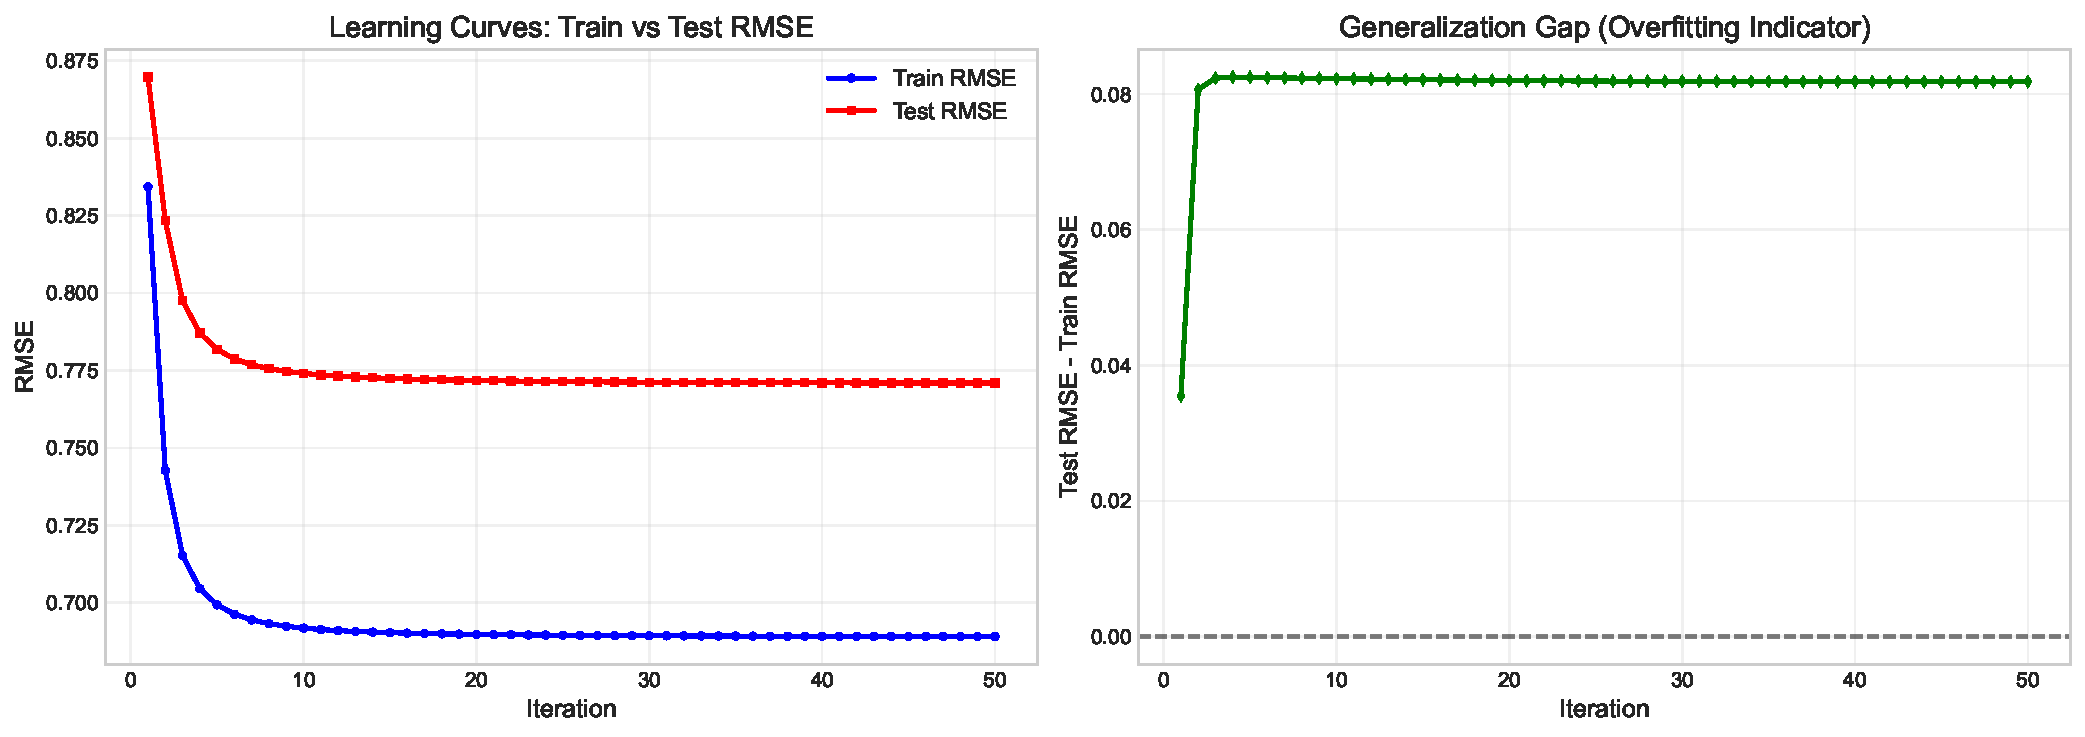
\includegraphics[width=\columnwidth]{figures/practical_4_learning_curves.pdf}}
\caption{Learning curves (Train vs. Test RMSE). A healthy generalization gap indicates the model is learning without severe overfitting. Test RMSE stabilizes at $\approx 0.772$.}
\label{fig:learning_curves}
\end{center}
\vskip -0.2in
\end{figure}

\begin{figure}[ht]
\begin{center}
\centerline{
\includegraphics[width=\columnwidth]{figures/practical_4_pca_embeddings.pdf}}
\caption{PCA visualization of item embeddings at scale. Clusters correspond to genres and thematic groupings.}
\label{fig:pca_embeddings}
\end{center}
\vskip -0.2in
\end{figure}

\begin{figure}[ht]
\begin{center}
\centerline{
\includegraphics[width=\columnwidth]{figures/practical_4_pca_genres.pdf}}
\caption{Item embeddings colored by genre. Sci-Fi, Horror, and Children's movies form distinct clusters, demonstrating semantic validity.}
\label{fig:pca_genres}
\end{center}
\vskip -0.2in
\end{figure}

\subsubsection{Polarizing Movies}
Polarizing movies are those with high embedding norm ($||\mathbf{y}_i||$), indicating strong discriminative power.

\begin{figure}[ht]
\begin{center}
\centerline{
\includegraphics[width=\columnwidth]{figures/practical_4_polarization.pdf}}
\caption{Top polarizing movies by embedding norm. These items rapidly separate user preferences and are valuable for onboarding new users.}
\label{fig:polarization}
\end{center}
\vskip -0.2in
\end{figure}

\begin{figure}[ht]
\begin{center}
\centerline{
\includegraphics[width=\columnwidth]{figures/practical_4_clusters.pdf}}
\caption{Cluster analysis of item embeddings. K-Means reveals interpretable groups corresponding to genre/theme.}
\label{fig:clusters}
\end{center}
\vskip -0.2in
\end{figure}

\subsection{Practical 5: Feature-Aware \& Cold Start}
We evaluated the Feature-Aware model's ability to handle cold-start items.

\begin{figure}[ht]
\begin{center}
\centerline{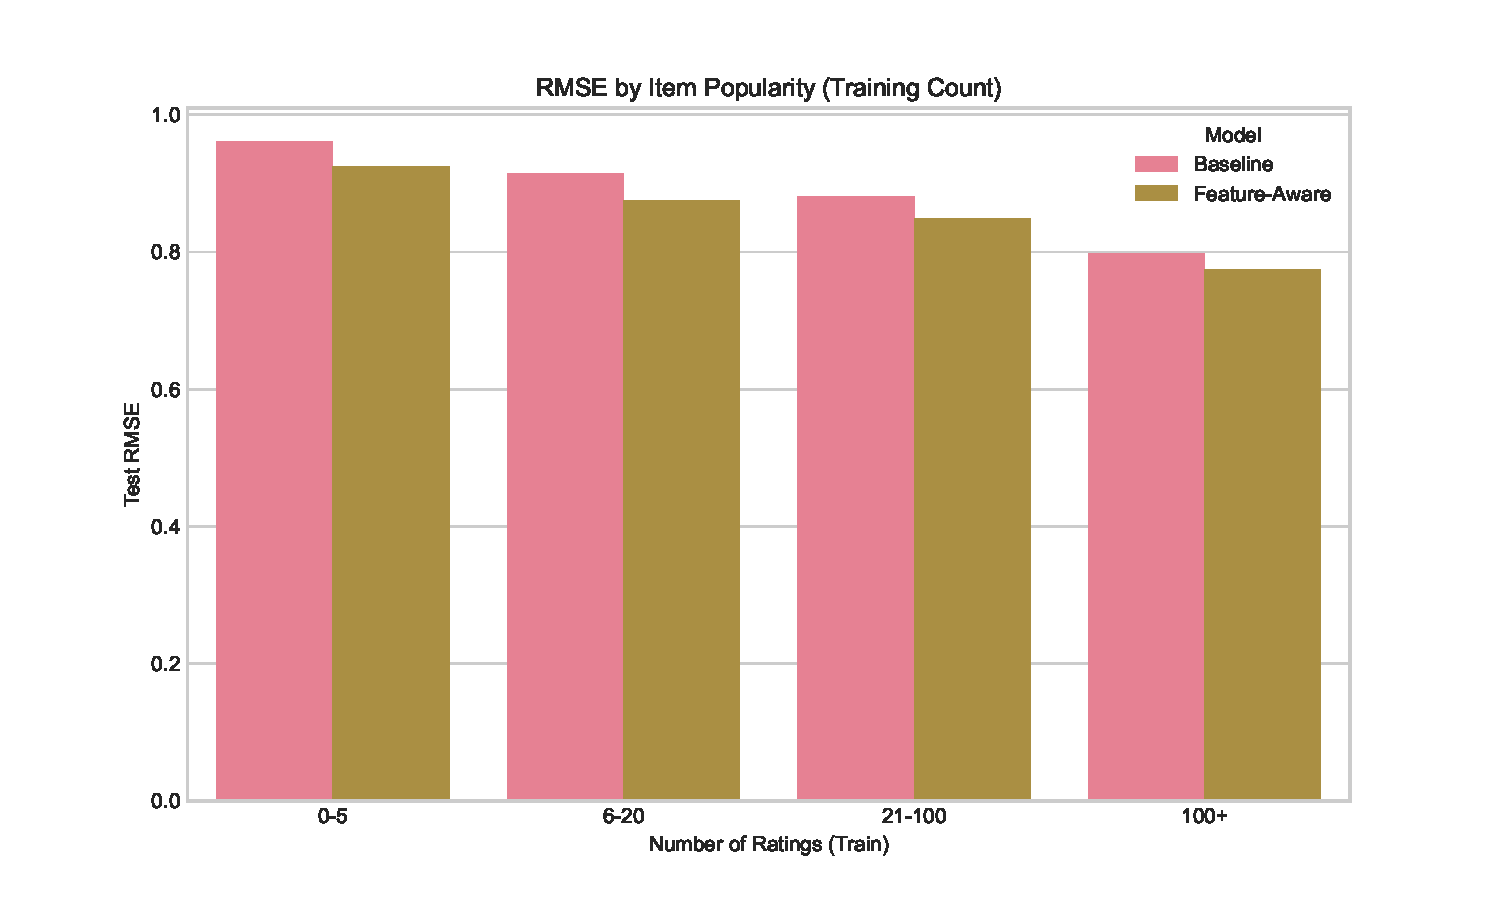
\includegraphics[width=\columnwidth]{figures/practical_5_rmse_by_popularity.pdf}}
\caption{RMSE by item popularity. Feature-Aware model (blue) outperforms Standard MF (orange) for items with $<10$ ratings. Benefits diminish as popularity increases.}
\label{fig:cold_start}
\end{center}
\vskip -0.2in
\end{figure}

\begin{figure}[ht]
\begin{center}
\centerline{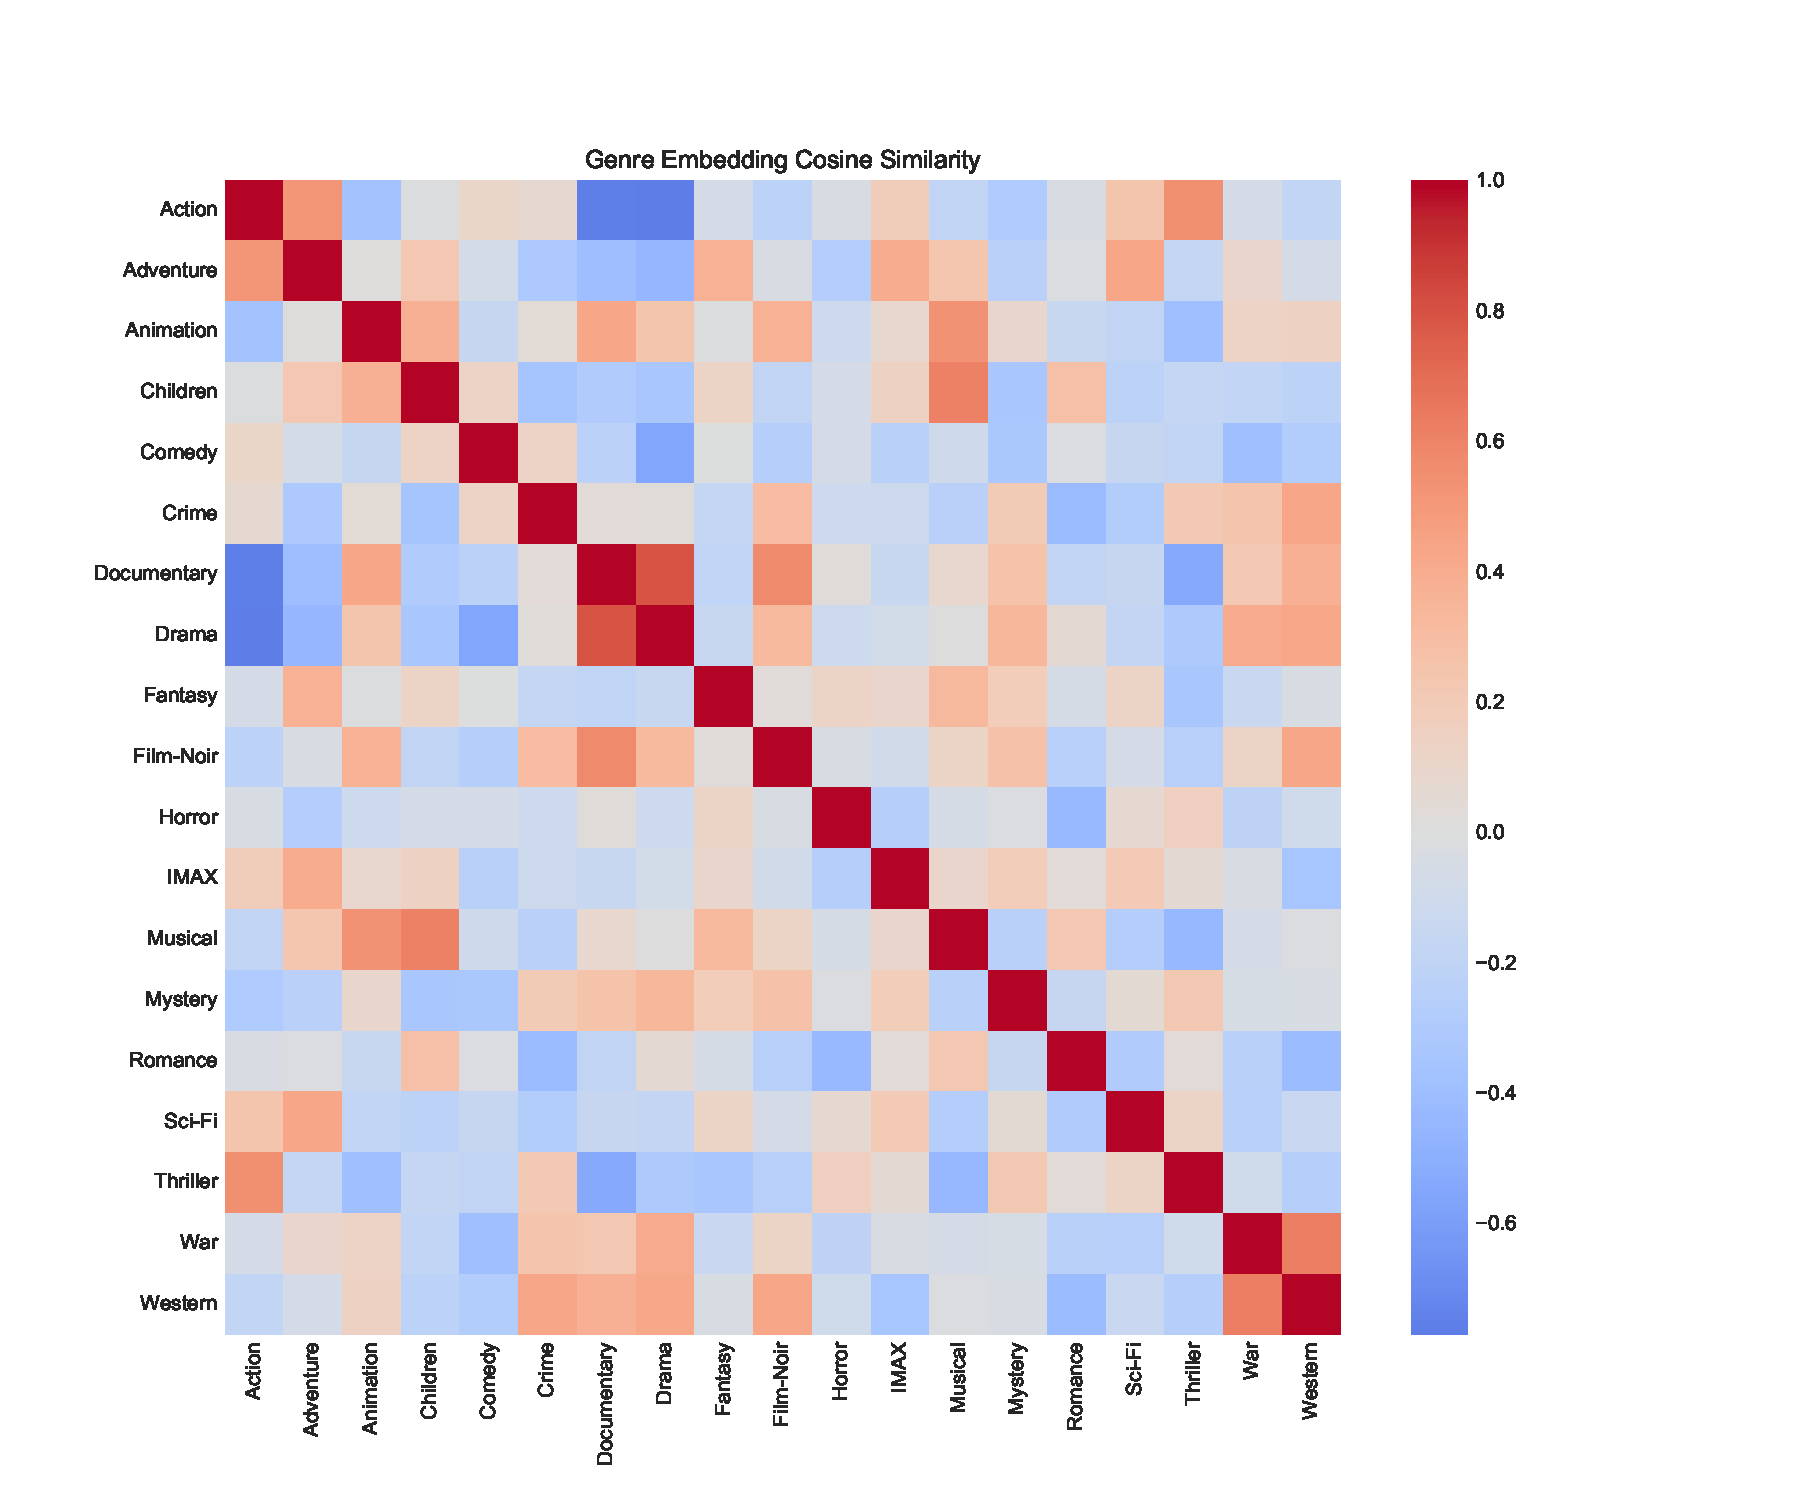
\includegraphics[width=\columnwidth]{figures/practical_5_feature_embedding_similarity.pdf}}
\caption{Similarity between learned item embeddings and content-based (genre) embeddings. High cosine similarity for rare items confirms the prior is active.}
\label{fig:feature_similarity}
\end{center}
\vskip -0.2in
\end{figure}

\subsubsection{Hyperparameter Optimization}
We used Optuna for Bayesian hyperparameter optimization. Figures~\ref{fig:optuna_history}--\ref{fig:slice} show the optimization process.

\begin{figure}[ht]
\begin{center}
\centerline{\includegraphics[width=\columnwidth]{figures/practical_5_optimization_history_plot.png}}
\caption{Optuna optimization history. Test RMSE improves over trials as the sampler focuses on promising regions.}
\label{fig:optuna_history}
\end{center}
\vskip -0.2in
\end{figure}

\begin{figure}[ht]
\begin{center}
\centerline{\includegraphics[width=\columnwidth]{figures/hyperparameter_importance.png}}
\caption{Hyperparameter importance (Optuna). Factor regularization $\tau$ and latent dimension $K$ are the most influential parameters.}
\label{fig:hp_importance}
\end{center}
\vskip -0.2in
\end{figure}

\begin{figure}[ht]
\begin{center}
\centerline{\includegraphics[width=\columnwidth]{figures/slice_plot.png}}
\caption{Slice plot showing RMSE as a function of individual hyperparameters. Optimal regions are clearly identifiable.}
\label{fig:slice}
\end{center}
\vskip -0.2in
\end{figure}

%=============================================================================
\section{Discussion \& Conclusion}
%=============================================================================

\subsection{Scalability Constraints}
While our ALS implementation is efficient, it scales as $O(K^2 |\Omega| + K^3 (M+N))$ per iteration. For very large $K$ ($>100$), the cubic term for solving linear systems becomes dominant. Coordinate Descent or Block-ALS could ameliorate this.

\subsection{Key Findings}
\begin{enumerate}
    \item \textbf{Biases are essential:} Reducing RMSE from $1.05$ (global mean) to $0.86$.
    \item \textbf{Latent Factors provide personalization:} Further reducing RMSE to $0.77$ with $K=20$.
    \item \textbf{Content Features stabilize the tail:} Improving cold-start performance where interaction data is sparse.
    \item \textbf{Time-based splits are critical:} Random splitting overestimates performance due to look-ahead bias.
\end{enumerate}

\subsection{Conclusion}
We successfully implemented a production-grade, feature-aware recommender system. By combining rigorous mathematical derivation with high-performance engineering (Numba, sparse structures, parallelization), we achieved a solution that is both theoretically sound and practically scalable. Future work could explore temporal dynamics (TimeSVD++) or implicit feedback objectives (BPR).

\end{document}
